% Options for packages loaded elsewhere
% Options for packages loaded elsewhere
\PassOptionsToPackage{unicode}{hyperref}
\PassOptionsToPackage{hyphens}{url}
\PassOptionsToPackage{dvipsnames,svgnames,x11names}{xcolor}
%
\documentclass[
  english,
  11pt,
]{article}
\usepackage{xcolor}
\usepackage[margin=25mm]{geometry}
\usepackage{amsmath,amssymb}
\setcounter{secnumdepth}{-\maxdimen} % remove section numbering
\usepackage{iftex}
\ifPDFTeX
  \usepackage[T1]{fontenc}
  \usepackage[utf8]{inputenc}
  \usepackage{textcomp} % provide euro and other symbols
\else % if luatex or xetex
  \usepackage{unicode-math} % this also loads fontspec
  \defaultfontfeatures{Scale=MatchLowercase}
  \defaultfontfeatures[\rmfamily]{Ligatures=TeX,Scale=1}
\fi
\usepackage{lmodern}
\ifPDFTeX\else
  % xetex/luatex font selection
\fi
% Use upquote if available, for straight quotes in verbatim environments
\IfFileExists{upquote.sty}{\usepackage{upquote}}{}
\IfFileExists{microtype.sty}{% use microtype if available
  \usepackage[]{microtype}
  \UseMicrotypeSet[protrusion]{basicmath} % disable protrusion for tt fonts
}{}
\makeatletter
\@ifundefined{KOMAClassName}{% if non-KOMA class
  \IfFileExists{parskip.sty}{%
    \usepackage{parskip}
  }{% else
    \setlength{\parindent}{0pt}
    \setlength{\parskip}{6pt plus 2pt minus 1pt}}
}{% if KOMA class
  \KOMAoptions{parskip=half}}
\makeatother
% Make \paragraph and \subparagraph free-standing
\makeatletter
\ifx\paragraph\undefined\else
  \let\oldparagraph\paragraph
  \renewcommand{\paragraph}{
    \@ifstar
      \xxxParagraphStar
      \xxxParagraphNoStar
  }
  \newcommand{\xxxParagraphStar}[1]{\oldparagraph*{#1}\mbox{}}
  \newcommand{\xxxParagraphNoStar}[1]{\oldparagraph{#1}\mbox{}}
\fi
\ifx\subparagraph\undefined\else
  \let\oldsubparagraph\subparagraph
  \renewcommand{\subparagraph}{
    \@ifstar
      \xxxSubParagraphStar
      \xxxSubParagraphNoStar
  }
  \newcommand{\xxxSubParagraphStar}[1]{\oldsubparagraph*{#1}\mbox{}}
  \newcommand{\xxxSubParagraphNoStar}[1]{\oldsubparagraph{#1}\mbox{}}
\fi
\makeatother


\usepackage{longtable,booktabs,array}
\newcounter{none} % for unnumbered tables
\usepackage{calc} % for calculating minipage widths
% Correct order of tables after \paragraph or \subparagraph
\usepackage{etoolbox}
\makeatletter
\patchcmd\longtable{\par}{\if@noskipsec\mbox{}\fi\par}{}{}
\makeatother
% Allow footnotes in longtable head/foot
\IfFileExists{footnotehyper.sty}{\usepackage{footnotehyper}}{\usepackage{footnote}}
\makesavenoteenv{longtable}
\usepackage{graphicx}
\makeatletter
\newsavebox\pandoc@box
\newcommand*\pandocbounded[1]{% scales image to fit in text height/width
  \sbox\pandoc@box{#1}%
  \Gscale@div\@tempa{\textheight}{\dimexpr\ht\pandoc@box+\dp\pandoc@box\relax}%
  \Gscale@div\@tempb{\linewidth}{\wd\pandoc@box}%
  \ifdim\@tempb\p@<\@tempa\p@\let\@tempa\@tempb\fi% select the smaller of both
  \ifdim\@tempa\p@<\p@\scalebox{\@tempa}{\usebox\pandoc@box}%
  \else\usebox{\pandoc@box}%
  \fi%
}
% Set default figure placement to htbp
\def\fps@figure{htbp}
\makeatother



\ifLuaTeX
\usepackage[bidi=basic,shorthands=off]{babel}
\else
\usepackage[bidi=default,shorthands=off]{babel}
\fi
\ifLuaTeX
  \usepackage{selnolig} % disable illegal ligatures
\fi


\setlength{\emergencystretch}{3em} % prevent overfull lines

\providecommand{\tightlist}{%
  \setlength{\itemsep}{0pt}\setlength{\parskip}{0pt}}



 


\makeatletter
\@ifpackageloaded{caption}{}{\usepackage{caption}}
\AtBeginDocument{%
\ifdefined\contentsname
  \renewcommand*\contentsname{Table of contents}
\else
  \newcommand\contentsname{Table of contents}
\fi
\ifdefined\listfigurename
  \renewcommand*\listfigurename{List of Figures}
\else
  \newcommand\listfigurename{List of Figures}
\fi
\ifdefined\listtablename
  \renewcommand*\listtablename{List of Tables}
\else
  \newcommand\listtablename{List of Tables}
\fi
\ifdefined\figurename
  \renewcommand*\figurename{Figure}
\else
  \newcommand\figurename{Figure}
\fi
\ifdefined\tablename
  \renewcommand*\tablename{Table}
\else
  \newcommand\tablename{Table}
\fi
}
\@ifpackageloaded{float}{}{\usepackage{float}}
\floatstyle{ruled}
\@ifundefined{c@chapter}{\newfloat{codelisting}{h}{lop}}{\newfloat{codelisting}{h}{lop}[chapter]}
\floatname{codelisting}{Listing}
\newcommand*\listoflistings{\listof{codelisting}{List of Listings}}
\makeatother
\makeatletter
\makeatother
\makeatletter
\@ifpackageloaded{caption}{}{\usepackage{caption}}
\@ifpackageloaded{subcaption}{}{\usepackage{subcaption}}
\makeatother
\usepackage{bookmark}
\IfFileExists{xurl.sty}{\usepackage{xurl}}{} % add URL line breaks if available
\urlstyle{same}
% fallback for those not using the hyperref driver hyperxmp:
\makeatletter
\@ifundefined{xmpquote}{\newcommand{\xmpquote}[1]{#1}}{}
\makeatother
\hypersetup{
  pdftitle={How local corrections repair global constraints},
  pdflang={en},
  colorlinks=true,
  linkcolor={blue},
  filecolor={Maroon},
  citecolor={Blue},
  urlcolor={Blue},
  pdfcreator={LaTeX via pandoc}}


\title{How local corrections repair global constraints}
\usepackage{etoolbox}
\makeatletter
\providecommand{\subtitle}[1]{% add subtitle to \maketitle
  \apptocmd{\@title}{\par {\large #1 \par}}{}{}
}
\makeatother
\subtitle{An executable five-moment step from the Navier--Stokes
construction}
\author{}
\date{2026-09-11}
\begin{document}
\maketitle


\textbf{A correction confined to a small region can still leave an
unwanted effect outside that region. Weighted integrals determine
whether those exterior tails disappear.} This installment shows how five
localized adjustments can cancel five prescribed integral discrepancies.

The previous articles made the momentum residual and oscillatory
transport concrete. We now return to a specific correction step in the
paper. Its positive-order axisymmetric profiles must preserve integral
constraints when extended away from the axis. Equations (5.14)--(5.16)
repair those constraints using two axial bumps and three angular bumps.
\href{https://cdn.openai.com/pdf/32d9f210-8b73-45e0-91bc-82a30aef8a9a/navier-stokes.pdf}{OpenAI,
Lemma 5.2, pages 50--52}

We implement that finite solve, choose explicit smooth bumps, and verify
the corrected integrals with separate quadrature. The five input
discrepancies are prescribed test values. They have \textbf{not} been
computed from a reconstructed inner solution, so this is stage A of D6:
a source-defined substep, rather than a completed order-one momentum
correction.

\subsection{Why does a local change leave a distant
tail?}\label{why-does-a-local-change-leave-a-distant-tail}

Consider the simple relation

\[
F(R)=\int_0^R g(s)\,ds,
\]

where \(g\) vanishes outside a bounded interval. Beyond that interval,
\(F\) becomes constant. It becomes zero there only if the \textbf{total
integral of \(g\) is zero}.

Adding a compactly supported \(g\) therefore does not automatically give
a compactly supported \(F\). An integral condition is needed.

The same issue occurs in the correction construction. Reconstructing
radial velocity, pressure, and stress requires integration. Five moments
are imposed so that those reconstructed quantities have the required
exterior behavior. The two integrated stress conditions use cylindrical
radial weights.
\href{https://cdn.openai.com/pdf/32d9f210-8b73-45e0-91bc-82a30aef8a9a/navier-stokes.pdf}{OpenAI,
Equations (5.9)--(5.12)}

We can understand and test the finite moment solve before evaluating the
entire flow.

\subsection{Five controls for five
discrepancies}\label{five-controls-for-five-discrepancies}

Let \(R=\sqrt{2X}\) denote the dimensionless profile radius. Add two
compact bumps to the axial coefficient \(U_n\) and three to the angular
coefficient \(E_n\):

\[
\delta U_n=\alpha_1b^U_1+\alpha_2b^U_2,\qquad
\delta E_n=\beta_1b^E_1+\beta_2b^E_2+\beta_3b^E_3.
\]

The bumps are nonnegative, have unit integral, and occupy disjoint
radial intervals. Their coefficients may have either sign. These are
signed corrections to velocity profiles, rather than the nonnegative
squared wave amplitudes used for covariance matching in D4.

Our explicit bump centered at \(c\) has halfwidth \(w\):

\[
b(R)=
\begin{cases}
\displaystyle\frac1{wZ}
\exp\!\left[-\frac1{1-((R-c)/w)^2}\right],&|R-c|<w,\\
0,&|R-c|\ge w,
\end{cases}
\]

where \(Z\) normalizes its integral. The bump and all its derivatives
vanish at the edges. We use centers \(2,3\) for the axial bumps and
\(4,5,6\) for the angular bumps, with halfwidth \(0.12\). These are
representative positive profile radii; they have not been located inside
the actual paper annulus.

\subsection{The required coefficients come from two small
systems}\label{the-required-coefficients-come-from-two-small-systems}

The reserved patch has the source form \(U_0=0\) and
\(E_0=e_*f(\eta)R^{-1-2\lambda}\). This makes the moment response split
into two blocks:

\[
(B_U)_{ij}=\int_0^\infty R^{p_i}b^U_j(R)\,dR,
\qquad (p_1,p_2)=(1,1-2\lambda),
\]

\[
(B_E)_{ij}=\int_0^\infty R^{s_i}b^E_j(R)\,dR,
\qquad (s_1,s_2,s_3)=(2,-2-2\lambda,-2\lambda).
\]

For scaled discrepancies \(\mathbf d_U,\mathbf d_E\), the repair is

\[
B_U\boldsymbol\alpha=-\mathbf d_U,\qquad
B_E\boldsymbol\beta=-\mathbf d_E.
\]

These are the two systems in Equation (5.16).
\href{https://cdn.openai.com/pdf/32d9f210-8b73-45e0-91bc-82a30aef8a9a/navier-stokes.pdf}{OpenAI,
pages 51--52}

We solve the systems directly rather than explicitly forming matrix
inverses. The baseline uses \(\lambda=0.1\),

\[
\mathbf d_U=(1,-0.4),\qquad
\mathbf d_E=(0.3,-0.2,0.1).
\]

The parameter \(\lambda\) here controls the reserved-patch power law. It
is distinct from the expansion-order notation \(\lambda_n=2nh\).

\begin{figure}

\centering{

\pandocbounded{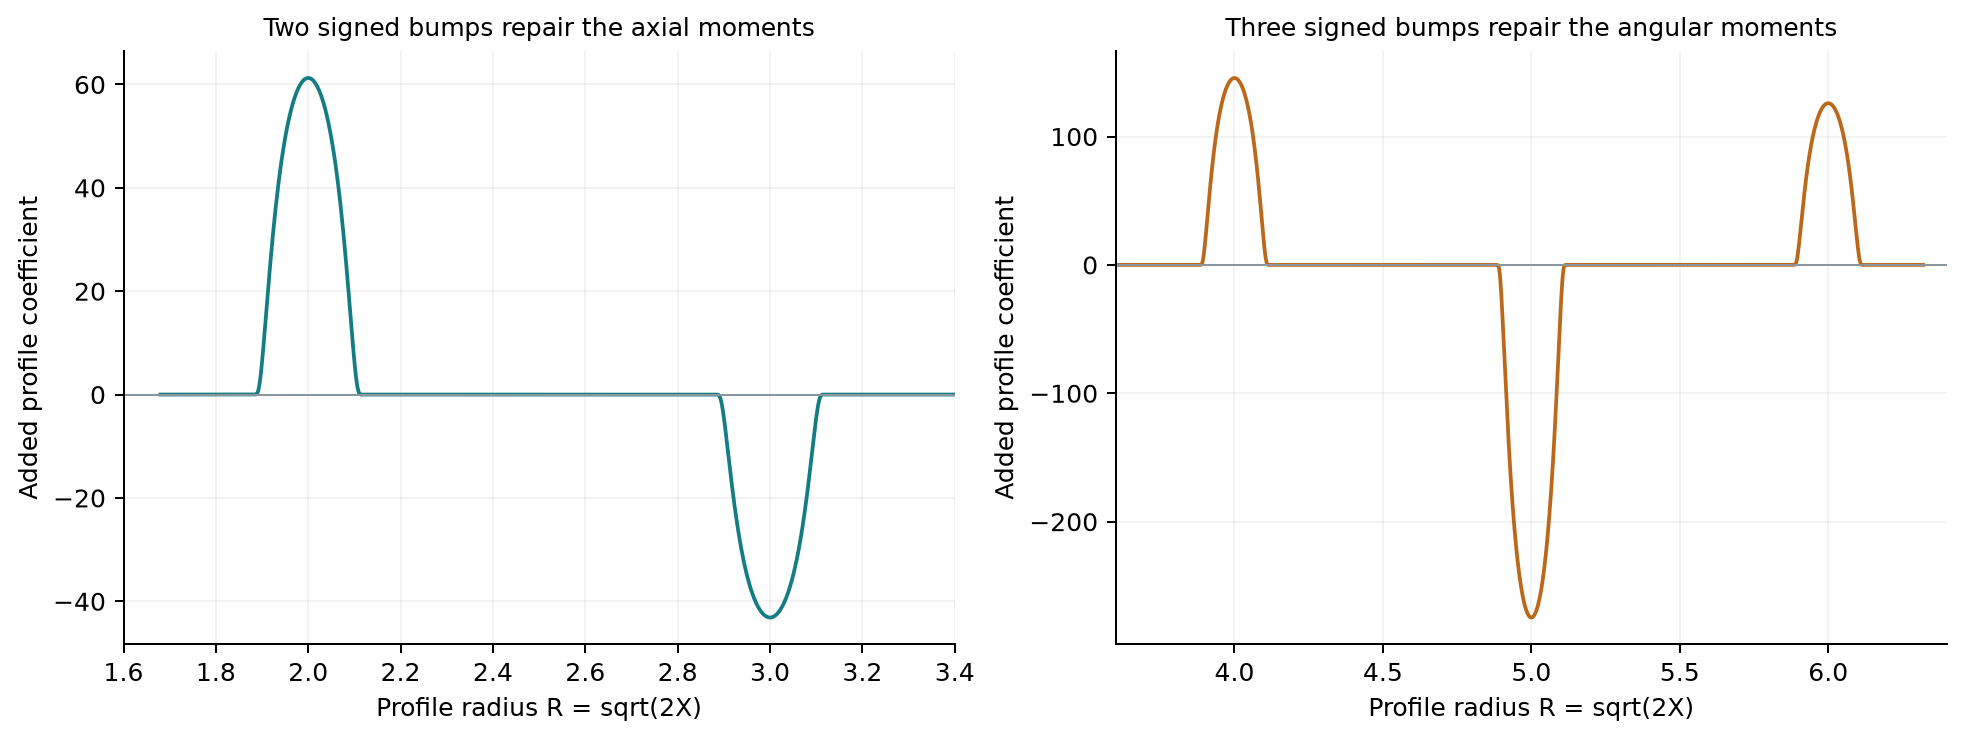
\includegraphics[keepaspectratio,alt={Two axial bumps and three angular bumps, with positive and negative coefficients, occupy disjoint intervals.}]{figures/01_local_profile_repair.png}}

}

\caption{\label{fig-profiles}The finite solve produces two signed axial
adjustments and three signed angular adjustments. Each bump is confined
to its chosen interval. The vertical axes show added profile
coefficients, not dimensional velocities or the complete corrected
profiles.}

\end{figure}%

\subsection{Check the integrals after applying the
correction}\label{check-the-integrals-after-applying-the-correction}

A small linear-system residual is useful, but it only checks consistency
with the matrix that was supplied to the solver. If the matrix integrals
are inaccurate, that solve can still give the wrong correction.

We therefore calculate the baseline matrix with quadrature order 96 and
evaluate the resulting moments again with order 384. The tests also
integrate the bump-weight products independently using adaptive
quadrature, including the pressure and momentum-flux factors from the
reserved patch.

For \(e_*f=1\), the original five moments corresponding to our inputs
are

\[
(m_1,m_2,m_3,m_4,m_5)=(1,0.3,-0.4,-0.4,-0.1).
\]

Each plotted remainder is divided by that moment's own initial
magnitude. This avoids combining moments with different weights into an
unexplained single norm.

\begin{figure}

\centering{

\pandocbounded{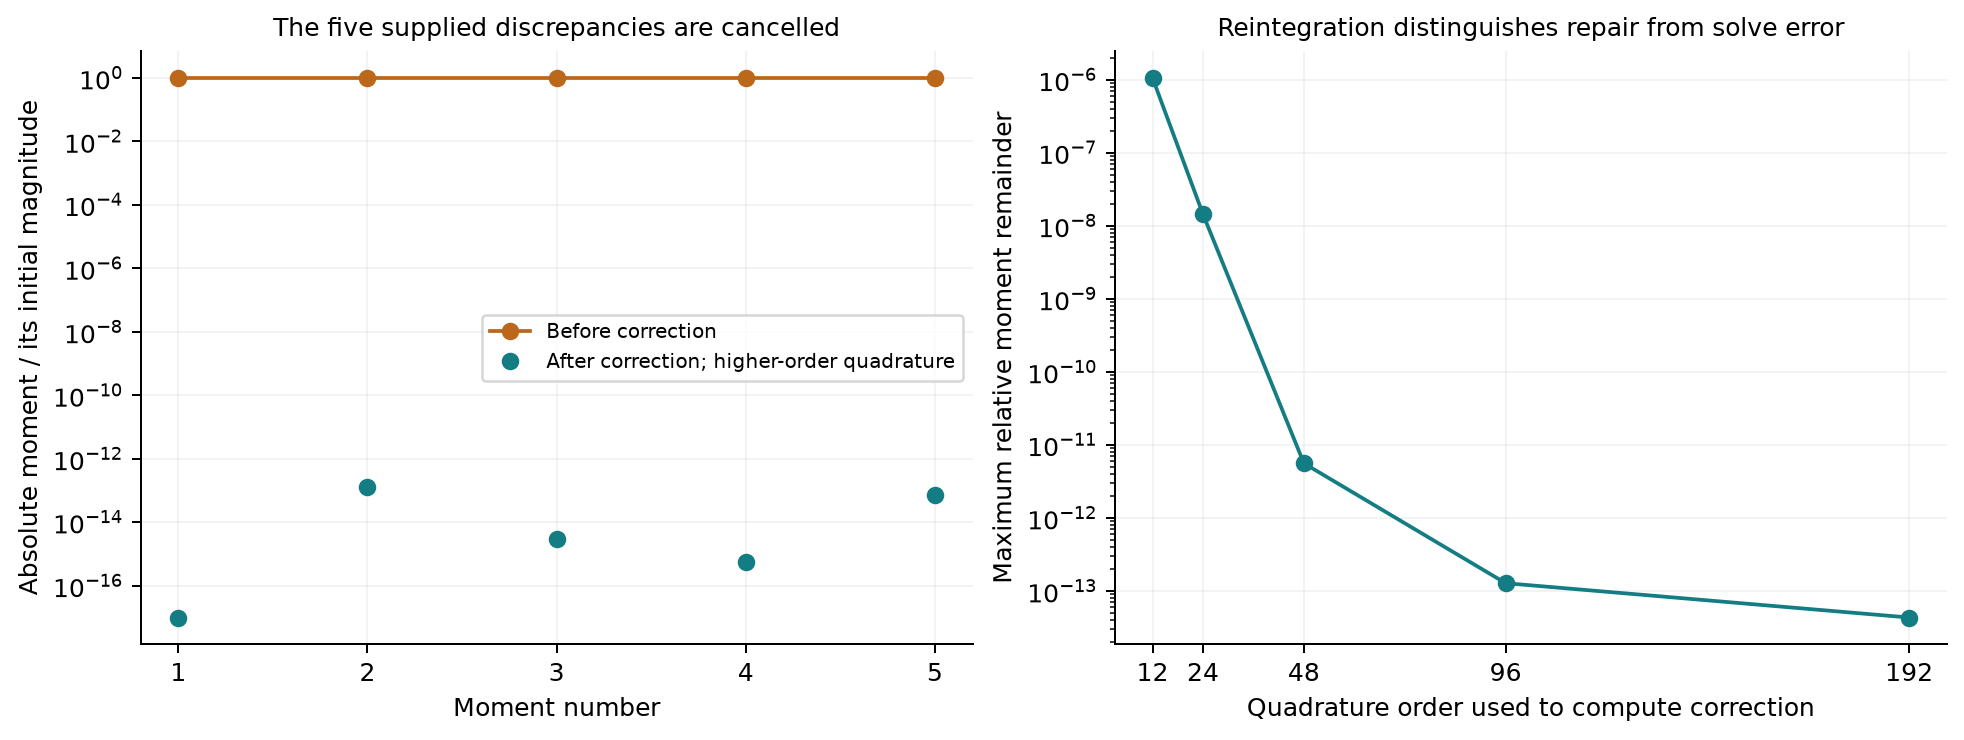
\includegraphics[keepaspectratio,alt={Five normalized moment discrepancies fall from one to near floating-point precision, with a separate quadrature-refinement check.}]{figures/02_moment_cancellation.png}}

}

\caption{\label{fig-moments}All five supplied discrepancies are reduced
close to floating-point precision after the correction. The right panel
recomputes the correction with different quadrature orders, then checks
every result using the higher reference order. These are moment
remainders, not Navier--Stokes momentum residuals.}

\end{figure}%

The largest absolute moment remainder is approximately \textbf{3.8e-14}.
The largest componentwise relative remainder is \textbf{1.3e-13}.

This verifies the selected integral repair for the declared inputs. It
does not verify the differential equations satisfied by an entire
corrected background.

\subsection{An invertible system can still be difficult to
compute}\label{an-invertible-system-can-still-be-difficult-to-compute}

The axial weights are \(R\) and \(R^{1-2\lambda}\). As \(\lambda\)
decreases toward zero, these two functions become nearly identical. The
two rows of \(B_U\) then become nearly dependent.

That has two separate consequences for our fixed test discrepancies. The
coefficients needed to satisfy both constraints become large, and
numerical errors in the moments become more strongly amplified.

\begin{figure}

\centering{

\pandocbounded{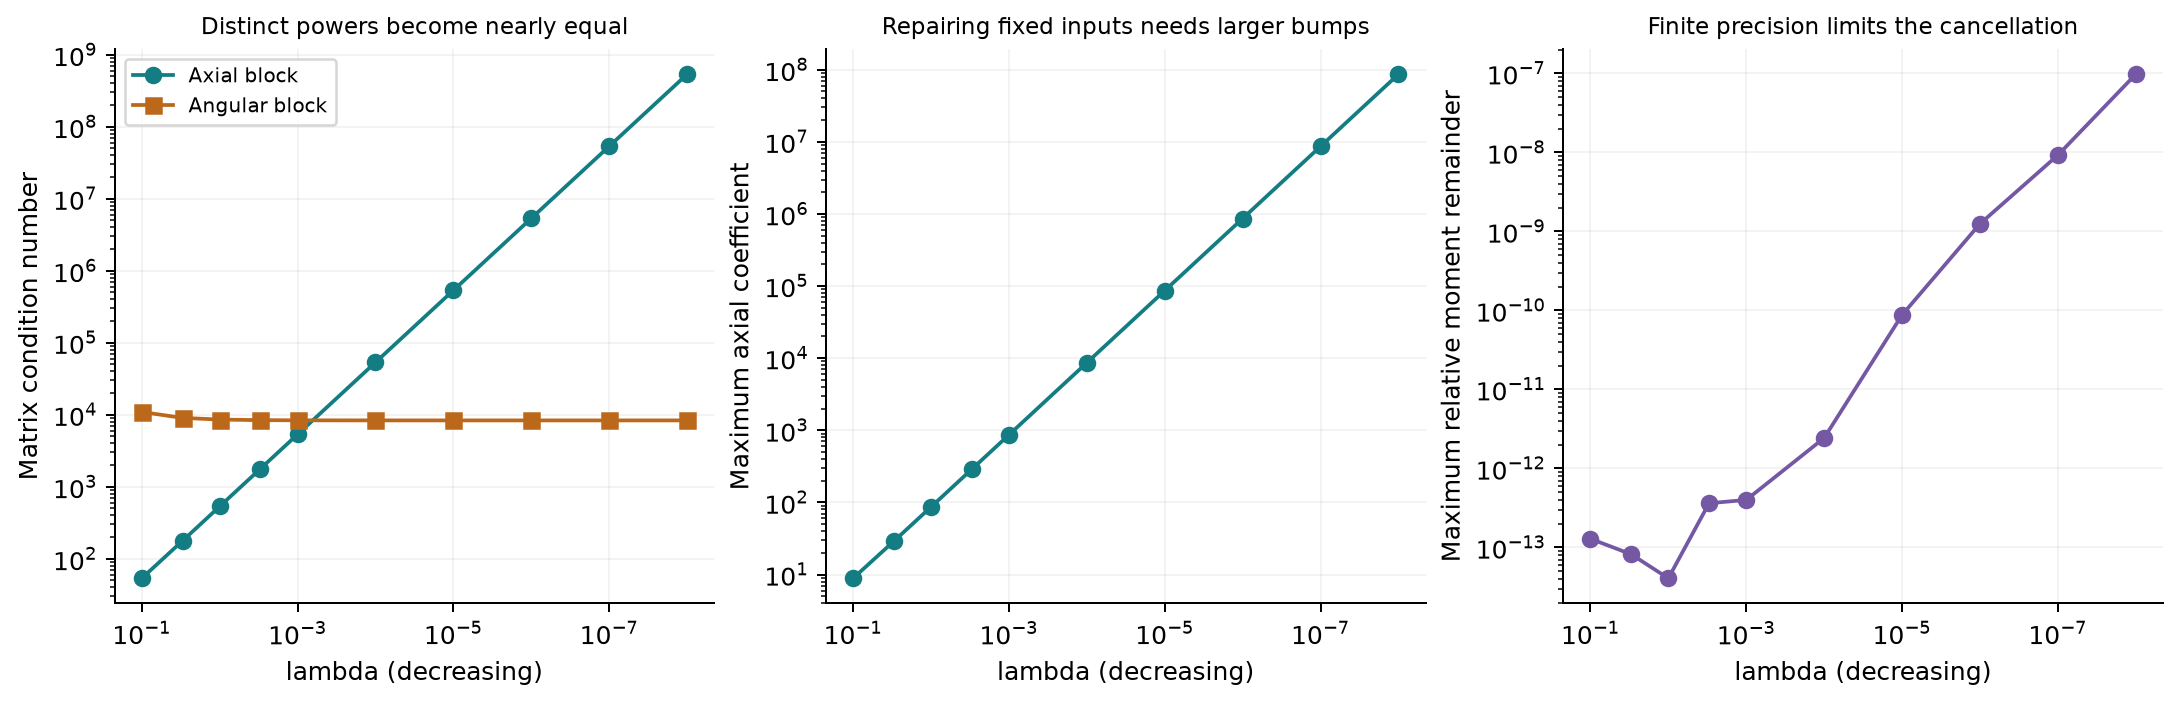
\includegraphics[keepaspectratio,alt={As lambda approaches zero, the axial matrix condition number and correction coefficients grow, and moment cancellation loses digits.}]{figures/03_conditioning_limit.png}}

}

\caption{\label{fig-conditioning}Decreasing the reserved-patch exponent
makes the axial moment matrix poorly conditioned, while the angular
block remains bounded over this scan. The fixed input discrepancies
require increasingly large axial coefficients. Reintegrated moment
remainders become larger in double precision. This is algebraic
sensitivity of the isolated solve, not dynamical stability of a flow.}

\end{figure}%

At \(\lambda=10^{-8}\), the axial condition number is about
\textbf{5.3e+08}, and the largest relative moment remainder is
approximately \textbf{9.7e-08} in this implementation.

Condition numbers depend on the chosen coordinates and scaling. The data
therefore also include the axial condition number after normalizing each
matrix row. Its deterioration persists because the rows are becoming
parallel.

The scan keeps the prescribed discrepancies fixed while changing
\(\lambda\). It does not construct a corresponding family of full paper
profiles. In particular, it establishes no instability of the proposed
Navier--Stokes solution. It identifies a numerical issue to check when
an actual profile supplies these discrepancies.

\subsection{What is still needed for a full correction
comparison?}\label{what-is-still-needed-for-a-full-correction-comparison}

The finite repair is ready to accept discrepancies from a future profile
calculation. The missing work lies upstream:

\begin{enumerate}
\def\labelenumi{\arabic{enumi}.}
\tightlist
\item
  Evaluate one joined leading profile, including its inner, annular, and
  exterior regions and the selected construction constants.
\item
  Solve the coupled first inner coefficient equations for the angular
  velocity, axial velocity, and pressure.
\item
  Extend that inner coefficient, compute its five actual discrepancies,
  and pass them to this repair.
\item
  Reconstruct the complete corrected fields and compare their momentum
  residuals on resolved physical-coordinate samples.
\end{enumerate}

The \href{implementation-ledger.md}{implementation ledger} lists the
source definitions and current status of those dependencies. The
published formalization repository was also inventoried; that check
found Lean source, but no Python/Julia/notebook or tabulated-profile
files of the inspected types. It was not a proof audit.

The numerical result here is a working, independently checked component
of the correction machinery. A reduction in these five integral
remainders must remain separate from the still-uncomputed reduction in
the full momentum residual.

The \href{../../code/d6_moment_correction/study.ipynb}{notebook},
\href{../../code/d6_moment_correction/parameters.json}{parameters}, and
\href{../../code/d6_moment_correction/data/}{CSV data} expose all
inputs, coefficients, and checks.




\end{document}
